As expected, in all cases the networks were asymmetric, 
the download bandwidth (the downlink) being significantly higher than the uploading
or uplink. This also explains the relationship between the uplink and ping,
presenting a major ping in the networks with lower uplink. The relationship
can be better be seen in the Figure \ref{fig:speeds}.

\begin{figure}[ht]
\centering
	%\rule{5.5cm}{7.1cm}
    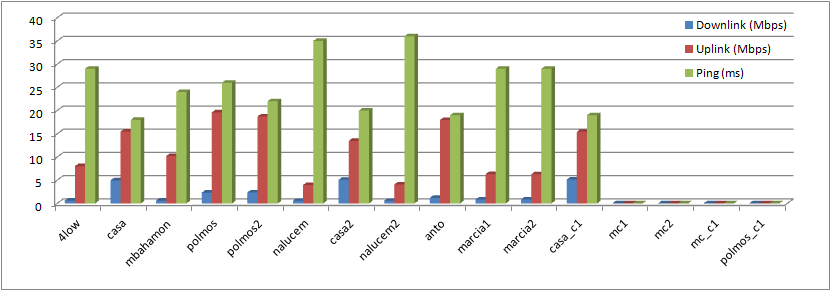
\includegraphics[width=0.9\textwidth]{img/speed_graph}
\caption{Speed and Pings based on Appendix \ref{app:bwmeasures}, Table \ref{table:speeds}}
\label{fig:speeds}
\end{figure}%

The Figure \ref{fig:speeds} also is a proof of the common missundersanding
about the how the ISP's promote high download speeds but with low uplink. Even
though most of the time home users download content, in order to keep a good
ratio the data needs to flow both ways, due to the way TCP
works, you need good communication in both directions. While in theory this
works without major problems, unfortunately in reality users download content
from different sources at once, and if we add new requirements like real-time  or on-demand applications and online games, we see that not only a
high-speed downlink is important.

Another important point is the growing need for higher bandwidth.
Unfortunately it is common to associate bandwidth with speed. Instead,
bandwidth is a measure of capacity, not how fast the network responds. So,
more capacity is only better if the existing latency is low. This may
explain why the tests performed in network tagged as \textit{``casa''} can have low pings
even when its capacity is close to the mean, but this network is through
fiber\footnote{In practice, fiber service have a propagation delay 10 times
faster than ASDL service}.

\begin{table}[ht]
\begin{center}
\begin{tabular}{|c||c|c||}
 \hline
& \multicolumn{2}{|c|}{Ratio (\%)} \\ \hline
Location	& Uplink		& Downlink \\ \hline \hline
casa\_w		& 99,00			& 103,20 \\ \hline
casa2\_w	& 101,80		&  89,73  \\ \hline
casa\_c		& 103,00		& 102,93  \\ \hline
marcia\_w	& 166,00		&  63,00  \\ \hline
marcia\_c	& 166,00		&  62,90  \\ \hline
sara\_w		& 112,00		&  54,50  \\ \hline
sara\_c		& 114,00		&  80,80 \\ \hline
polmos\_w	& 116,00		&  49,03  \\ \hline
polmos2\_w 	& 117,00		&  46,80  \\ \hline
nalucem\_w	& 114,00		&  99,25  \\ \hline
nalucem2\_w & 112,00		& 101,50  \\ \hline
mbahamon\_w & 120,00		& 102,10  \\ \hline
4low\_w	 	& 120,00		&  80,30  \\ \hline
hidalgo\_w 	& 119,00		&  89,80  \\ \hline
\end{tabular}
\caption[Speed Test: Variation ratio of offered vs measured speed ]{Variation ratio of offered vs measured speed.}
\label{table:ratiospeed}
\end{center}
\end{table}

The $\sim12ms$ ping were also not obtained, but the values ​​are still within
the acceptable range around the $\sim26ms$. These values ​​may be due to
factors such as congestion, conditions on the server, or the processing time
information. The variation of the ratio between the measured and the bandwidth
contracted is of 80\%, which is only 6\% less than the spected
value\footnote{Details of the provider and bandwidths can be found on Appendix
\ref{app:bwmeasures}, Table \ref{table:comparative}}.

Further analysis is needed to determinate how the bandwidth is related with
the Bufferbloat, but it is clear that less the bandwidth, higher the ping, but
it can not be stated the oppossite, higher the bandwidth, less the ping
becouse it also depends on how fast the network is and the effects in the
latency \cite{main:ref:3}.
